\documentclass[9pt,twocolumn,twoside]{osajnl}
\journal{ol} % Choose journal (ao, aop, josaa, josab, ol, pr)
% See template introduction for guidance on setting shortarticle option
\setboolean{shortarticle}{true}
% \documentclass[11pt,twocolumn,twoside]{osajnl}
\usepackage{caption,subcaption,graphicx,overpic,tikz,tkz-tab,verbatim,multirow,booktabs,siunitx,amsmath,amssymb,bm,mathtools,threeparttable,color,enumitem,listingsutf8,url,xcolor,etaremune,bibentry,textcomp,mathpazo,geometry,lastpage,fancyhdr,float,epstopdf,bm,upgreek,lineno,siunitx}
\linenumbers

\captionsetup[subfigure]{position=top}
% \setlength{\abovecaptionskip}{0pt} 
% \setlength{\belowcaptionskip}{0pt} 

\newcommand{\op}[1]{\ensuremath{\mathcal{#1}}}

%%%%%%%%%%%%%%%%%%%%%%%%%%%%%%%%%%%%%%%%%%%%%%%%%%%%%%%%%%%%%%%%%%%%
\title{Volumetric imaging by complex holographic deconvolution}

\author[1]{Ni Chen}
\author[2]{Peng Xia}
\author[3]{Edmund Y. Lam}
\author[1,*]{Byoungho Lee}

\affil[1]{Department of Electrical and Computer Engineering,
Seoul National University, Seoul 08826, Korea}
\affil[2]{Research Institute for Measurement and Analytical Instrumentation, National Metrology Institute of Japan, National Institute of Advanced Industrial Science and Technology, Tsukuba, Ibaraki 305-8568, Japan}
\affil[3]{Department of Electrical and Electronic Engineering, The University of Hong Kong, Pokfulam, Hong Kong}

\affil[*]{Corresponding author: byoungho@snu.ac.kr}

%% To be edited by editor
% \dates{Compiled \today}

%\ociscodes{(140.3490) Lasers, distributed feedback; (060.2420) Fibers, polarization-maintaining;(060.3735) Fiber Bragg gratings.}

%% To be edited by editor
% \doi{\url{http://dx.doi.org/10.1364/XX.XX.XXXXXX}}

\graphicspath{{./figure/}}

\begin{abstract}
We propose a volumetric imaging through three-dimensional holographic deconvolution approach. Both simulation and experimental results show our method works perfectly for overlapped objects with continues and discrete depth.

\end{abstract}

\setboolean{displaycopyright}{true}

\begin{document}

\maketitle

%====================================================================
\section{Introduction}\label{sec_intro}
Holography is regarded as a perfect technique for both three-dimensional~(3D) imaging~\cite{Chen2018Sensors} and display~\cite{Hong2011AO}, because it records the wavefront of 3D objects, including both amplitude and phase.
The object wavefront can be encoded into an intensity image through interforometrical approaches, or can be obtained directly or indirectly with digital processing approaches, such as optical scanning holography~(OSH)~\cite{Poon2009JOSK} and phase-shift holography~(PSH)~\cite{Yamaguchi2008OaPN}. 
In this letter, we focus on the complex holograms, i.e., holograms like OSH and PSH.

Even though holography records the 3D information, it can hardly been used for imaging directly. 
From the 3D holograms, one can do sectional reconstruction easily, the main problem is that a large residue signal from the undesired object section remains, which is often called the defocus noise, usually hindered the object information. 
To improve this, methods using Wiener filter~\cite{Kim2006AO}, Wigner distribution~\cite{Kim2008AO}, and inverse imaging~\cite{Lam2009AO,Zhang2010JOSA} have been developed.
However none of them can reconstruct a whole 3D volume, especially for overlapped 3D objects. On the contrary, we propose a method that can reconstruct 3D structure effectively, including objects that have continues-like depth, and of partially and completely overlapping.
To our best acknowledge, this is the first that can reconstruct a totally overlapped 3D objects.

%====================================================================
\section{Method}\label{sec_method}
Suppose $r=(x,y)$ is the lateral coordinates. When a 3D object $o(r,z)$ is illuminated by a plane wave along the optical axis, the result object wavefront at a point of $(r_h, z_h)$ can be represented as a convolution of the object transmittance function with the impulse response of free-space propagation~\cite{Goodman2005}
\begin{equation}
\begin{aligned}
u(r_h,z_h) 
& = \iiint o(r,z) \frac{\exp\left(jk\sqrt{(r_h-r)^2 + (z_h-z)^2}\right)}{\sqrt{(r_h-r)^2 + (z_h-z)^2}} d r dz, \\
& = o(r,z) \otimes \frac{\exp\left(jk\sqrt{r^2 + z^2}\right)}{\sqrt{r^2 + z^2}},
\label{eq_3ddiffr}
\end{aligned}
\end{equation}
where $k$ is the wave number, $\otimes$ is the convolution operator, and $h(r,z)=\frac{\exp(jk\sqrt{r^2 + z^2})}{\sqrt{r^2 + z^2}}$ is the point spread function~(PSF). 
Both OSH and PSH can obtain the object wavefront directly or indirectly.
The digital reconstruction, thus can be obtained by back-propagation of the  wavefront $u(r_h,z_h)$. The back-propagation involves a convolution of the hologram with the complex conjugate PSF $h^*(r, z_r)$, the sectional reconstruction at the corresponding position is 
\begin{equation}
\begin{aligned}
o'(r,z_r) 
& = u(r_h,z_h)\otimes h^*(r,z_r) \delta(z_r-z_h) , \\
& = o(r,z_r)\vert_{z_r=z_h} + o(r,z_r) \otimes h(r, z_h-z_r) \vert_{z_r \neq z_h}
\label{eq_3ddiffr_inv}
\end{aligned}
\end{equation}
It is clear that the reconstructed sectional image contains an unwanted second term~(the second term), and usually submerges the object signal seriously, especially for a 3D object with complicated structure. Sectional reconstruction usually solve this as an inverse problem~\cite{Zhang2010JOSA}. 

% It should be noted that the desired object information only exists in the real part of the sectional reconstruction.  

Don't like the previous techniques, we build the 3D model of the wave propagation, and conduct the complex operation.

Eq.~(\ref{eq_3ddiffr}) can also be written as
\begin{equation}
\Im\left\{u(r,z_h)\right\} = \Im\left\{o(r,z)\right\} \Im\left\{h(r,z)\right\} \label{eq_3dholo_ft}
\end{equation}
where $\Im$ is the operator of Fourier transform.
We represent the lexicographically ordered 2D hologram $\Im\left\{u(r,z)\right\}$ as a vector of $\mathbf{U(z)}$. 
Similarly, $\Im\left\{o(r,z)\right\}$ is represented as a vector $\mathbf{O}(r,z)$, $\Im\left\{h(r,z)\right\}$ is represented as $\mathbf{H}(k_r, z)$.
The product of $\Im\left\{o(r,z)\right\} \mathbf{H}(k_r, z)$ becomes $\mathbf{H}(r,z)\mathbf{O}(r,z)$.
Considering the complexity property of the holography, we let  $\mathbf{U}=\begin{bmatrix}\mathbf{U}_R & \mathbf{U}_I \end{bmatrix}^T$, and $\mathbf{H}(z)=\begin{bmatrix}\mathbf{H}_R(z) & \mathbf{H}_I(z) \end{bmatrix}^T$, where the subscript $_R$ and $_I$ means real and imaginary operators of a complex value.

Eq.~(\ref{eq_3dholo_ft}) thus can be written as
\begin{equation}
% \begin{bmatrix}
\mathbf{U} \\ 
% \mathbf{U}_I 
% \end{bmatrix}
=\begin{bmatrix}
\mathbf{H}(z_1) & \dots & \mathbf{H}(z_n) \\
% \mathbf{H}_I(z_1) & \dots & \mathbf{H}_I(z_n) 
\end{bmatrix}
\begin{bmatrix}
\mathbf{O}(z_1) \\ 
\vdots  \\
\mathbf{O}(z_n)\\  
\end{bmatrix} + \mathbf{n}
\end{equation}
where $\mathbf{n}$ is the noise. As the second term of Eq.~(\ref{eq_3ddiffr_inv}) shows, the noise should be multidimensional white Gaussian distribution.

To reconstruct object sections, we need to recover the object vector $\mathbf{O}$ given the measurement in $\mathbf{U}$, which is
an inverse problem. A broadly used method is to find the solution to the following minimization problem,
% This is an inverse problem under convex, non-smooth regularizes, the unconstrained form is
\begin{equation}
\mathbf{O}_{est} = \min_\mathbf{O} \frac{1}{2} \lVert \mathbf{H}\mathbf{O} - \mathbf{G} \rVert _2^2  + \tau \Phi(\mathbf{O})
\label{eq_O_est}
\end{equation}
where $\tau \in R_+$ is the regularization parameter. $\Phi$ is the total variation (TV) constraints, and
\begin{equation}
\Phi(\mathbf{O})=\sum_z\sum_x\sum_y\lvert \nabla (\mathbf{O})\rvert
\label{eq_TV}
\end{equation}
Therefore, the cost function of this minimization problem consists of two terms, one for the measurement domain error and the other for the regularization of the minimizer. 
The two-step iterative shrinkage/thresholding~(TwIST) algorithm is used to solve Eq.~(\ref{eq_O_est}).
%
%Algorithms can be included using the commands as shown in algorithm \ref{alg:euclid}.
%
%\begin{algorithm}
%\caption{Euclid’s algorithm}\label{alg:euclid}
%\begin{algorithmic}[1]
%\Procedure{Euclid}{$a,b$}\Comment{The g.c.d. of a and b}
%\State $r\gets a\bmod b$
%\While{$r\not=0$}\Comment{We have the answer if r is 0}
%\State $a\gets b$
%\State $b\gets r$
%\State $r\gets a\bmod b$
%\EndWhile\label{euclidendwhile}
%\State \textbf{return} $b$\Comment{The gcd is b}
%\EndProcedure
%\end{algorithmic}
%\end{algorithm}

\subsection{Normalization of the complex hologram}

%====================================================================
\section{Results}\label{sec_results}

Figure \ref{fig_sim} shows the simulation results. 
Several objects of various 3D structures were used to verify the feasibility of our method. The color-bar show the transmittance of the object. 
The wavelength of the illumination light source is \SI{633}{\nano\meter}, ..... 

The first column shows the objects used in the simulations, where the second column shows the top and side view of the objects, which are used to show the occlusion of the objects.

In Fig.~\ref{fig_sim}(a), the transmittance of the object is a conical helix function, therefore there is no overlapped portion along the optical axis. 
Fig.~\ref{fig_sim}(b) shows an example where the object is partially overlapped,
and Fig.~\ref{fig_sim}(c) is a circular helix, its totally overlapped along the optical axis.
The complex holograms are obtained by propagating the 3D objects along the optical axis with a distance. 
The third columns of each sub figures show the back-propagation volumetric reconstruction of the objects. The signals are totally hided in the reconstructed volume. 
The right most column show the reconstructions with our proposed method, the 3D are clearly resolved. It should be mentioned that both the partially and totally overlapped information were reconstructed perfectly.

\begin{figure}[H]
\centering
\fbox{
\begin{subfigure}[b]{0.95\columnwidth}
  \centering
    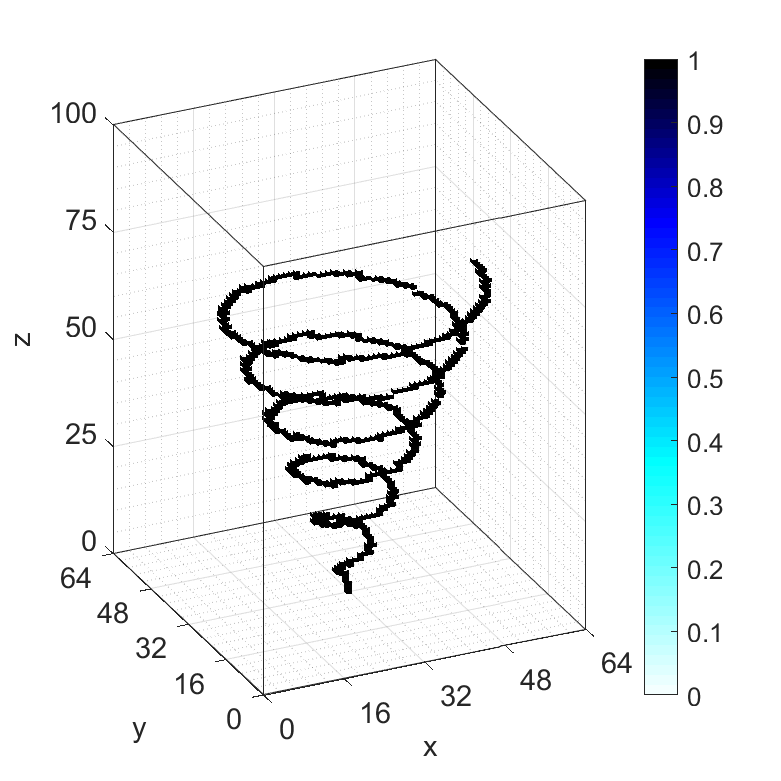
\includegraphics[width=0.27\columnwidth]{conhelix}
    \begin{minipage}[b]{0.13\columnwidth}
      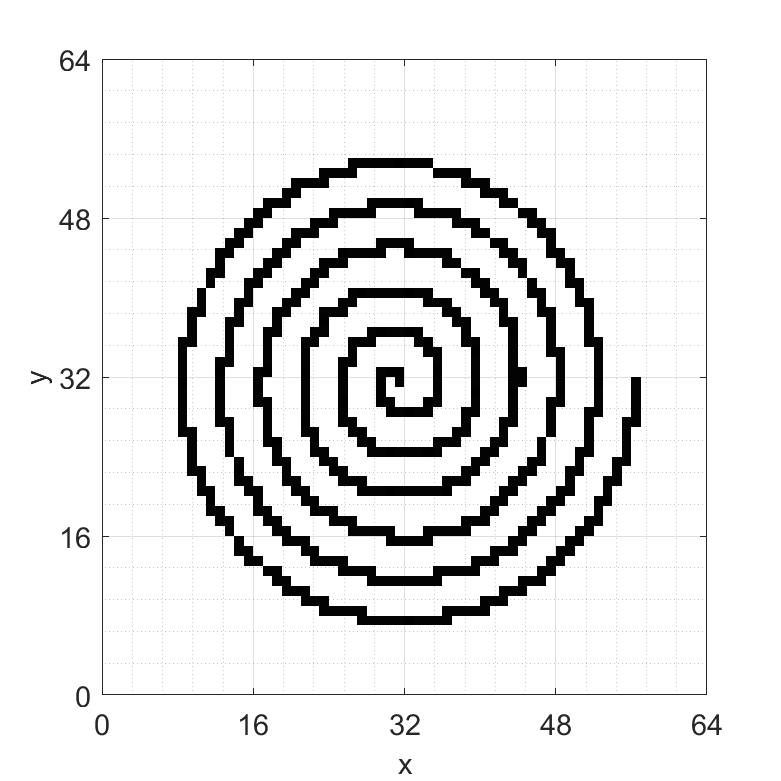
\includegraphics[width=1\columnwidth]{conhelix_top}
      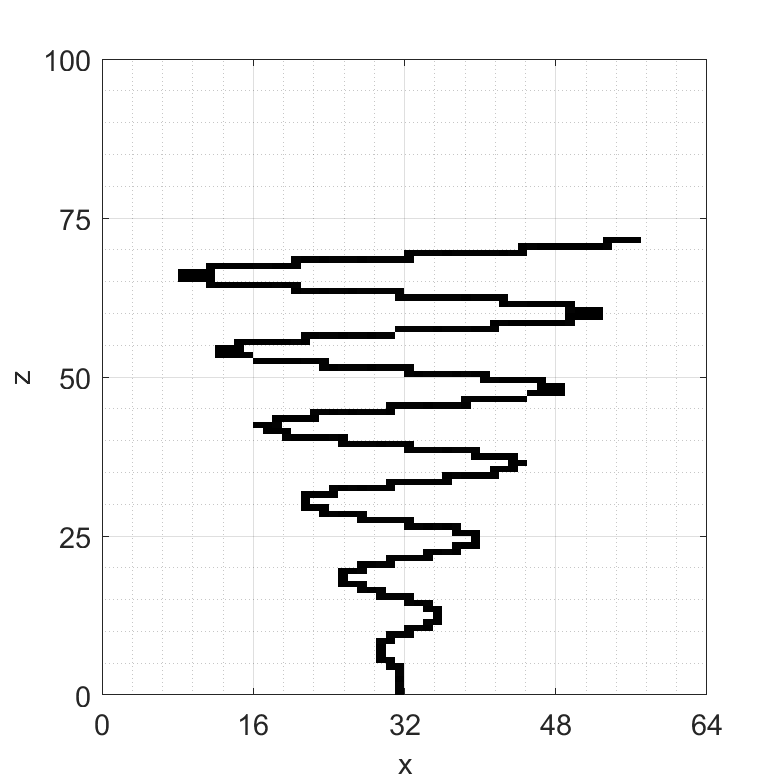
\includegraphics[width=1\columnwidth]{conhelix_side}
    \end{minipage}
    % \begin{minipage}[b]{0.13\columnwidth}
    %   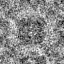
\includegraphics[width=1\columnwidth]{conhelix_complex_holo}
    %   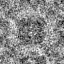
\includegraphics[width=1\columnwidth]{conhelix_complex_holo}
    % \end{minipage}
    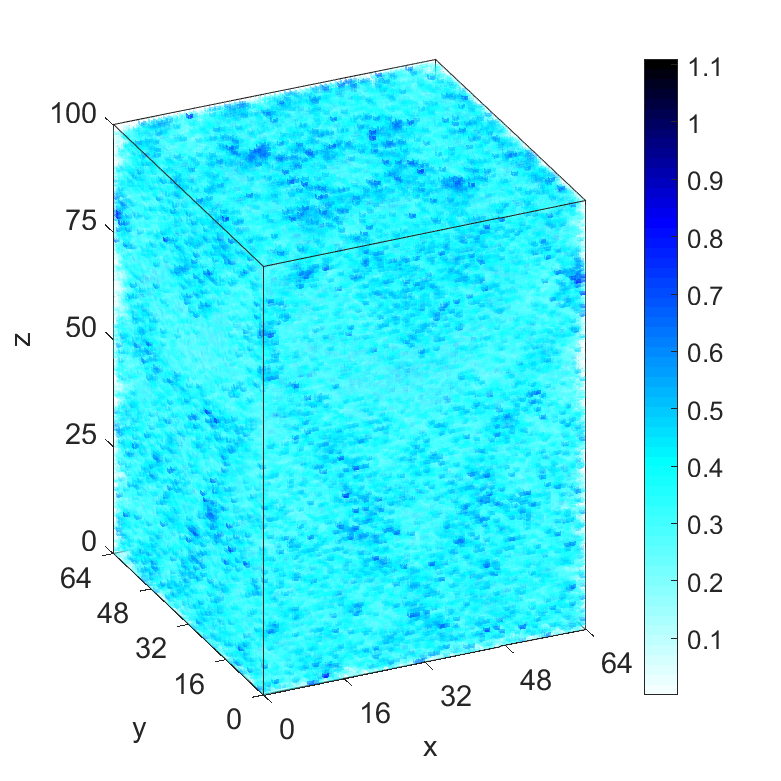
\includegraphics[width=0.27\columnwidth]{conhelix_complex_BP_3d}
    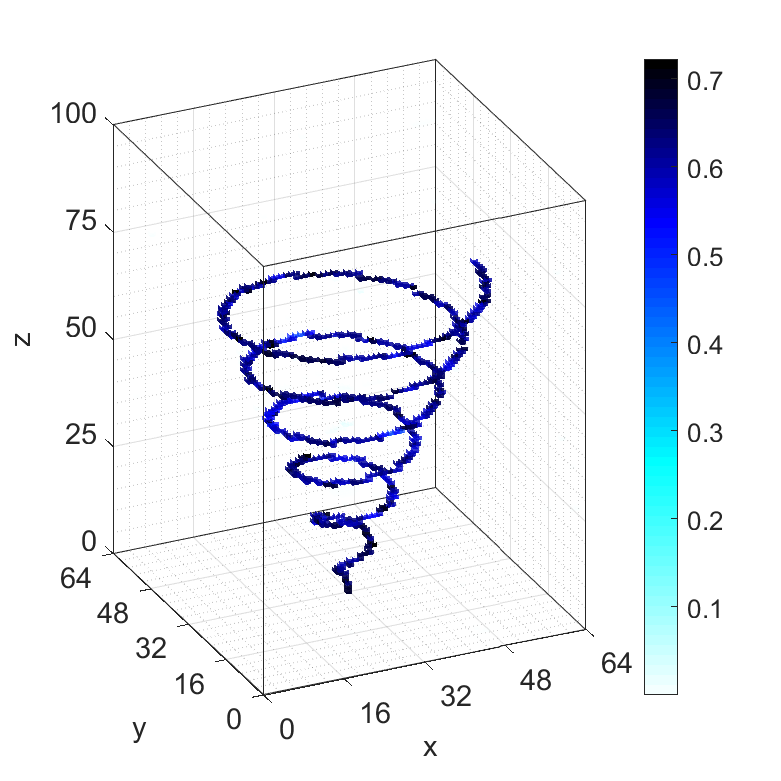
\includegraphics[width=0.27\columnwidth]{conhelix_complex_TwIST_3d}
    \caption{}
    % \vspace{-8pt}
\end{subfigure}}

\fbox{
\begin{subfigure}[b]{0.95\columnwidth}
 \centering
    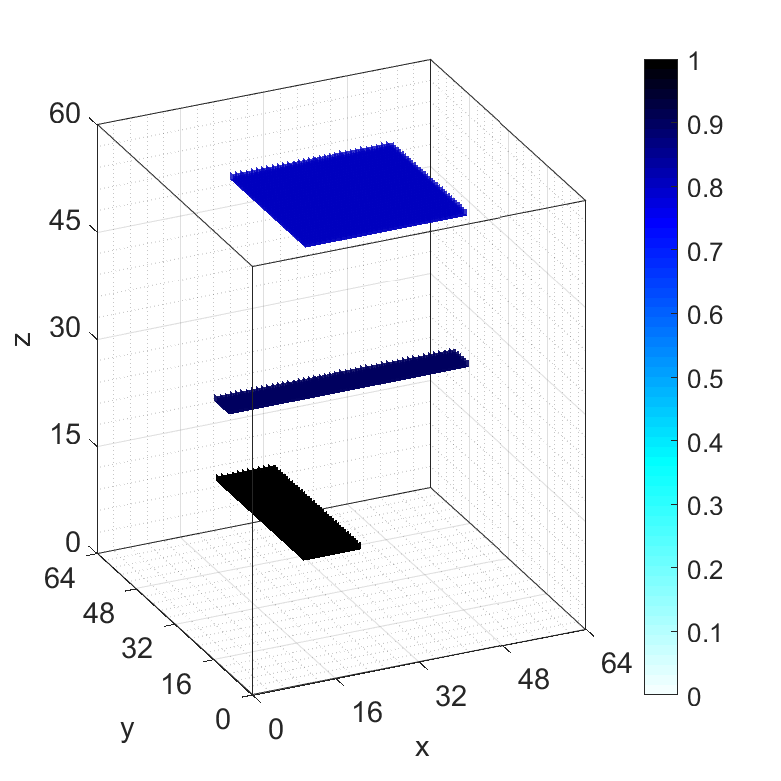
\includegraphics[width=0.27\columnwidth]{overlap}
    \begin{minipage}[b]{0.13\columnwidth}
      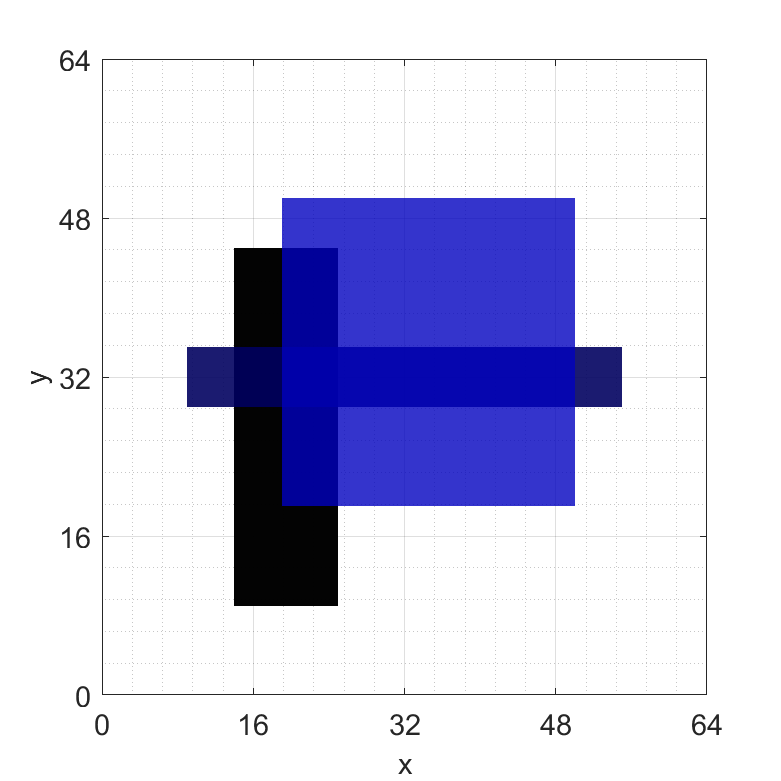
\includegraphics[width=1\columnwidth]{overlap_top}
      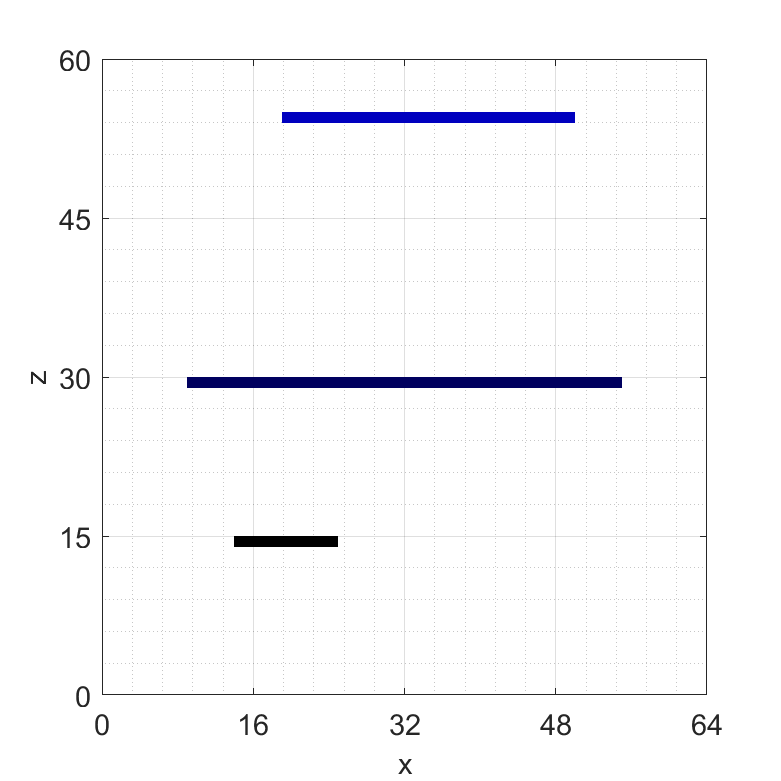
\includegraphics[width=1\columnwidth]{overlap_side}
    \end{minipage}
    % \begin{minipage}[b]{0.12\columnwidth}
    %   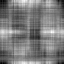
\includegraphics[width=1\columnwidth]{overlap_complex_holo}
    %   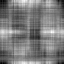
\includegraphics[width=1\columnwidth]{overlap_complex_holo}
    % \end{minipage}
    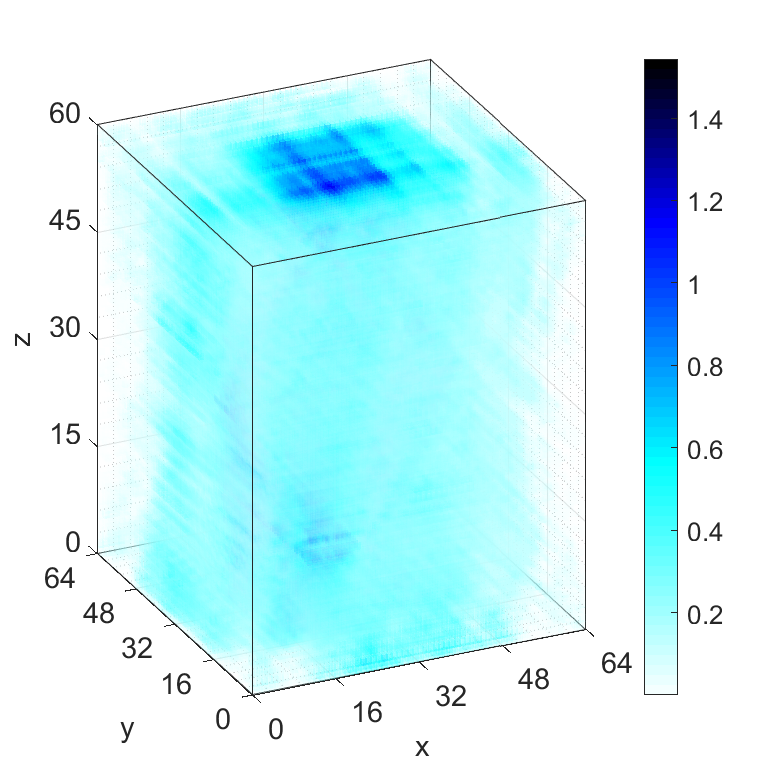
\includegraphics[width=0.27\columnwidth]{overlap_complex_BP_3d}
    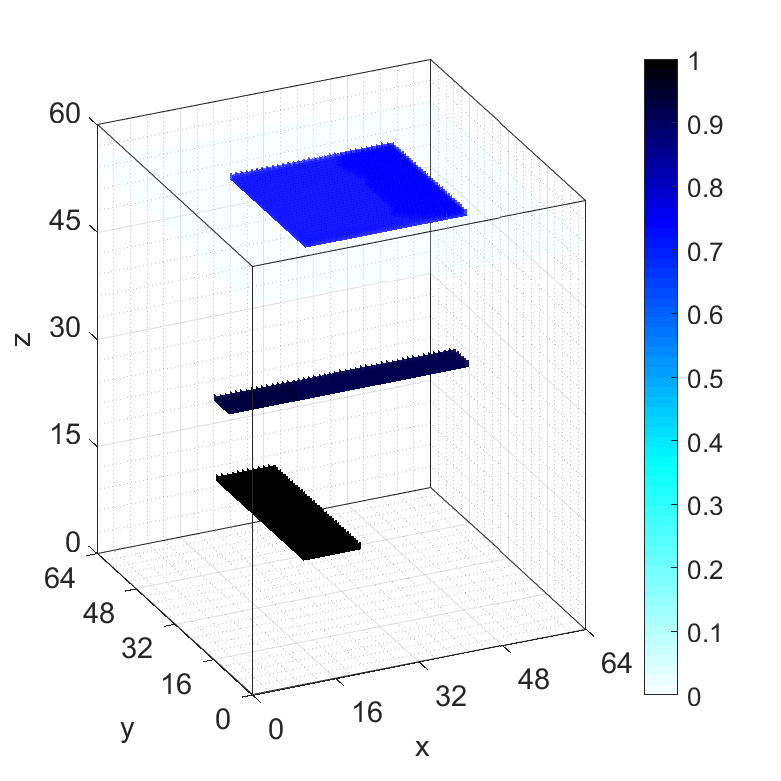
\includegraphics[width=0.27\columnwidth]{overlap_complex_TwIST_3d}
    \caption{}
    % \vspace{-8pt}
\end{subfigure}}

\fbox{
\begin{subfigure}[b]{0.95\columnwidth}
 \centering
    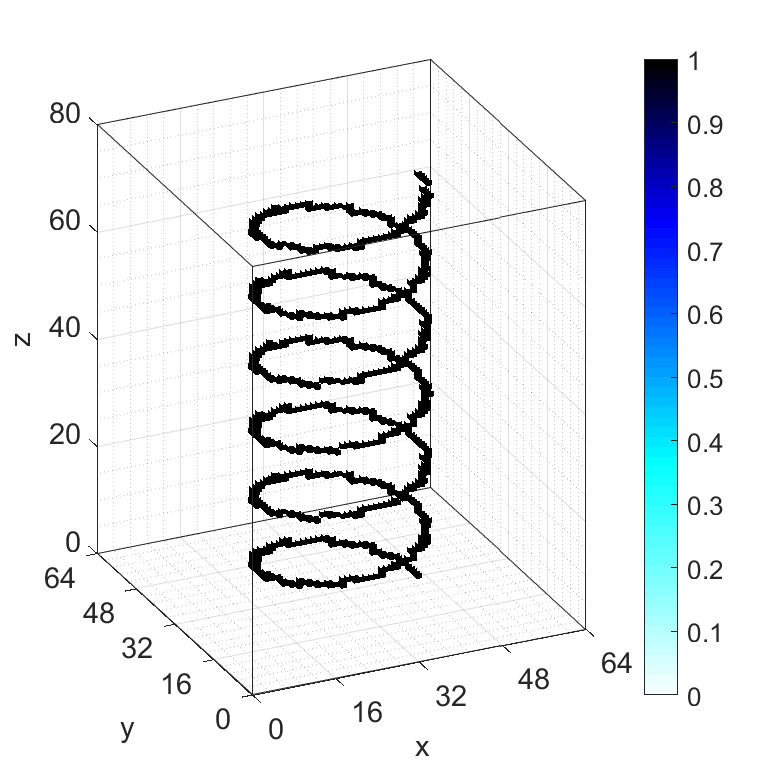
\includegraphics[width=0.27\columnwidth]{cirhelix}
    \begin{minipage}[b]{0.13\columnwidth}
      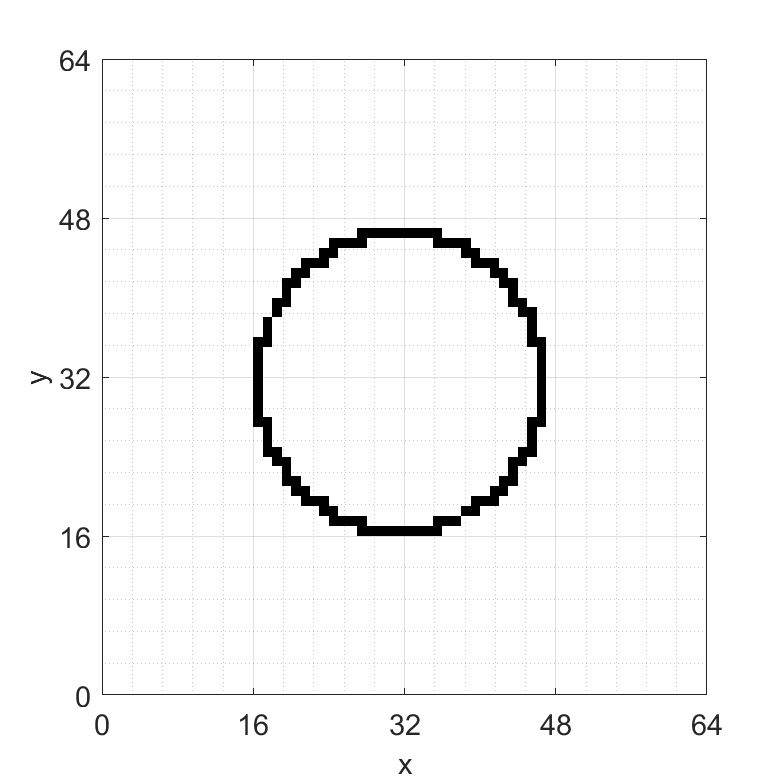
\includegraphics[width=1\columnwidth]{cirhelix_top}
      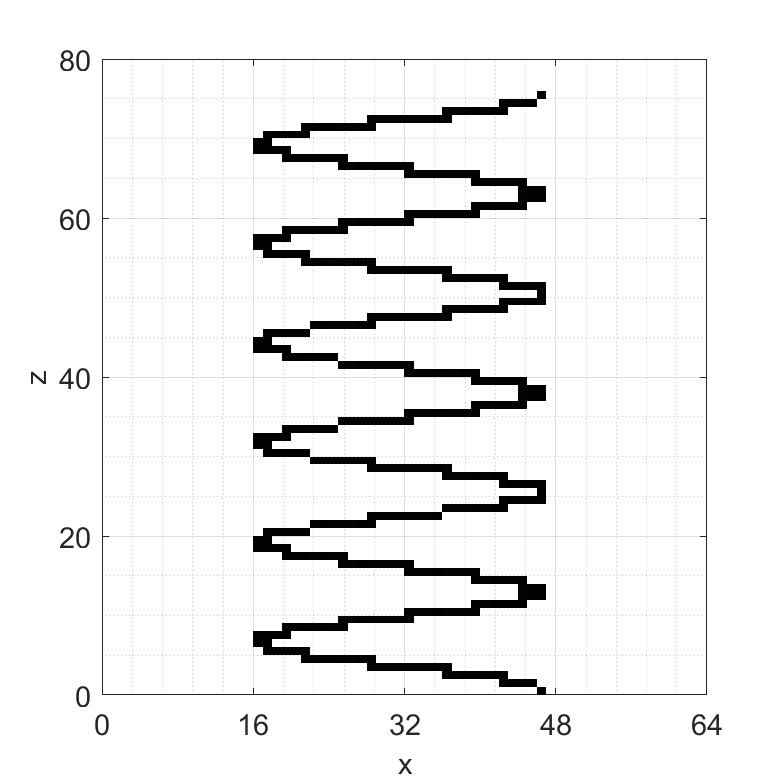
\includegraphics[width=1\columnwidth]{cirhelix_side}
    \end{minipage}
    % \begin{minipage}[b]{0.12\columnwidth}
    %   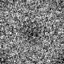
\includegraphics[width=1\columnwidth]{cirhelix_complex_holo}
    %   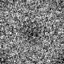
\includegraphics[width=1\columnwidth]{cirhelix_complex_holo}
    % \end{minipage}
    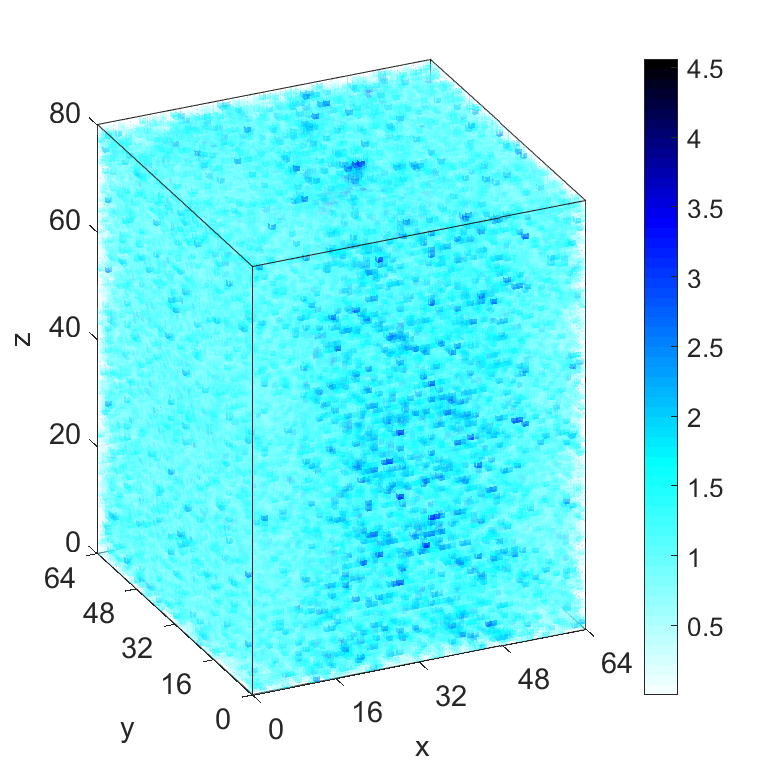
\includegraphics[width=0.27\columnwidth]{cirhelix_complex_BP_3d}
    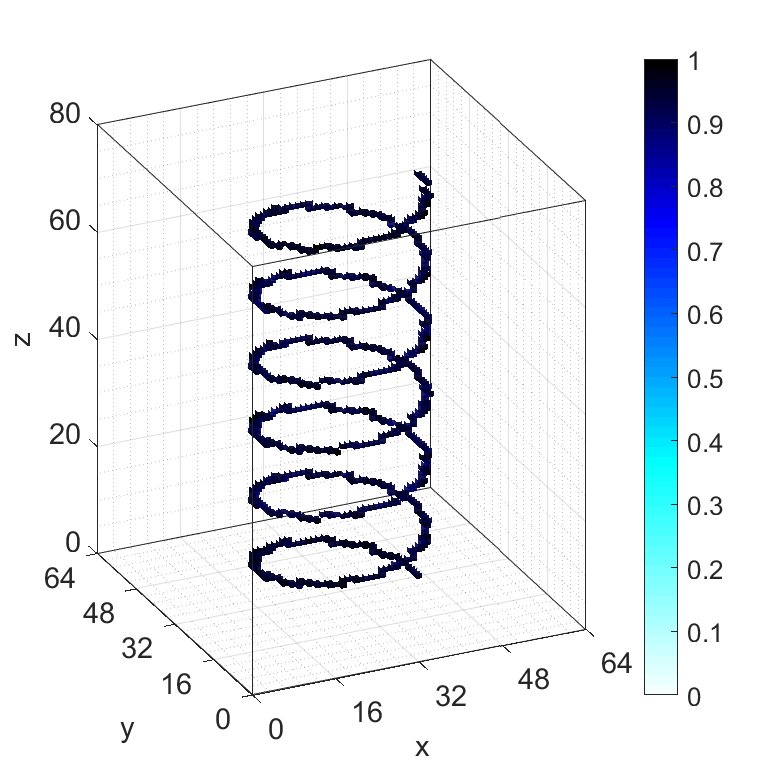
\includegraphics[width=0.27\columnwidth]{cirhelix_complex_TwIST_3d}
    \caption{}
\end{subfigure}}
\caption{Simulation (Gaussian noise with 35db)}
\label{fig_sim}
\end{figure}

Figure~\ref{fig_exp} shows the experimental reconstructions from phase-shifting holograms.

\begin{figure}[H]
\fbox{
\begin{subfigure}[b]{0.95\columnwidth}
  \centering
  \begin{minipage}[b]{0.15\columnwidth}
    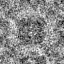
\includegraphics[width=1\columnwidth]{conhelix_complex_holo}
    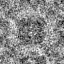
\includegraphics[width=1\columnwidth]{conhelix_complex_holo}
    \end{minipage}
    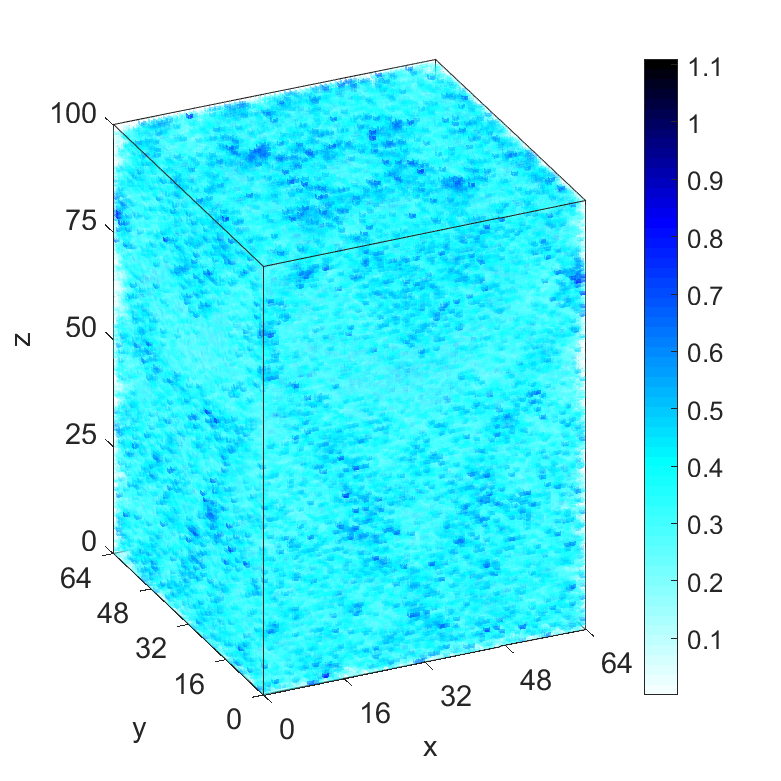
\includegraphics[width=0.33\columnwidth]{conhelix_complex_BP_3d}
    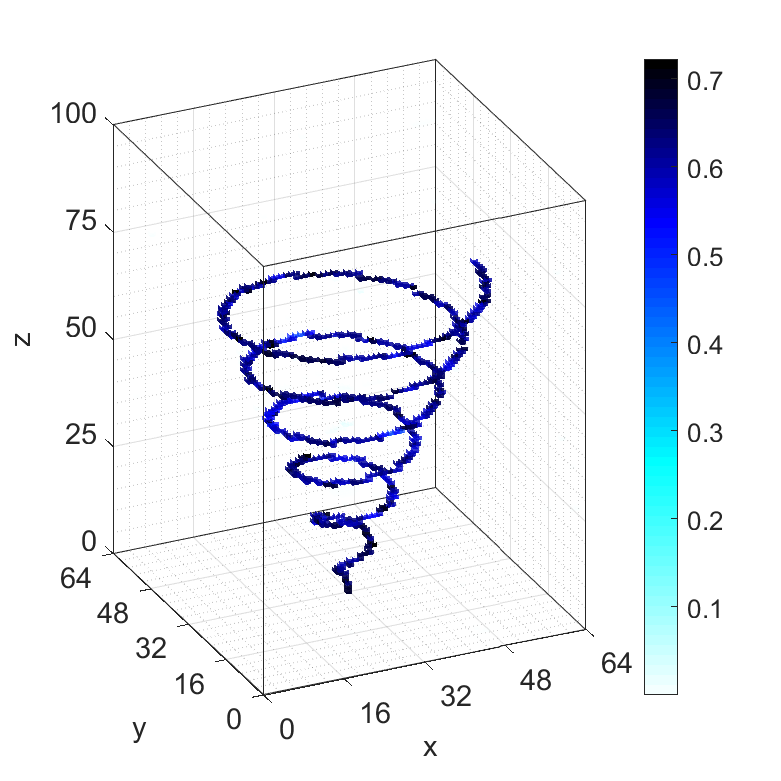
\includegraphics[width=0.33\columnwidth]{conhelix_complex_TwIST_3d}
    \caption{}
\end{subfigure}}

\fbox{
\begin{subfigure}[b]{0.95\columnwidth}
  \centering
  \begin{minipage}[b]{0.15\columnwidth}
    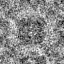
\includegraphics[width=1\columnwidth]{conhelix_complex_holo}
    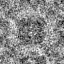
\includegraphics[width=1\columnwidth]{conhelix_complex_holo}
    \end{minipage}
    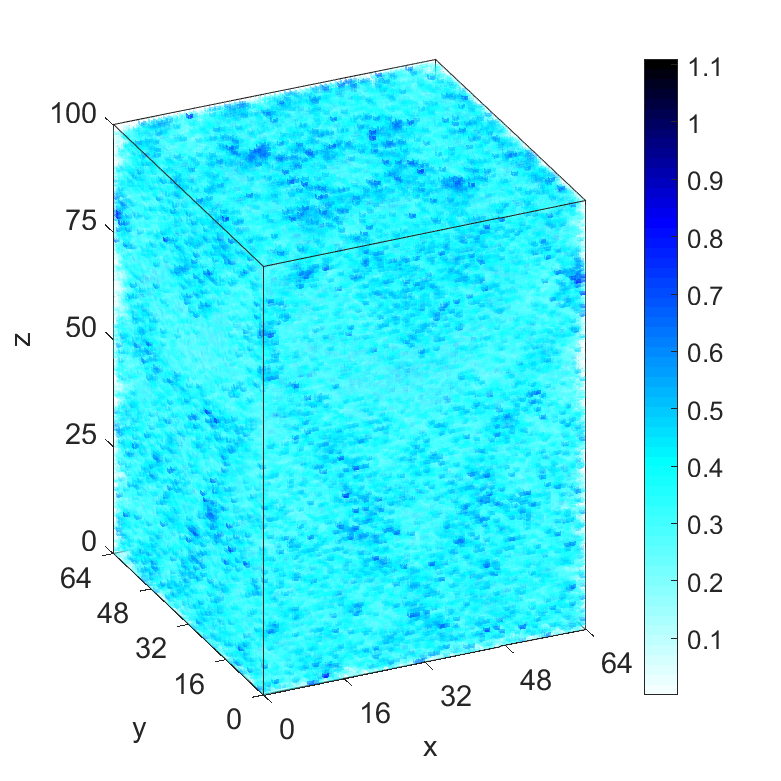
\includegraphics[width=0.33\columnwidth]{conhelix_complex_BP_3d}
    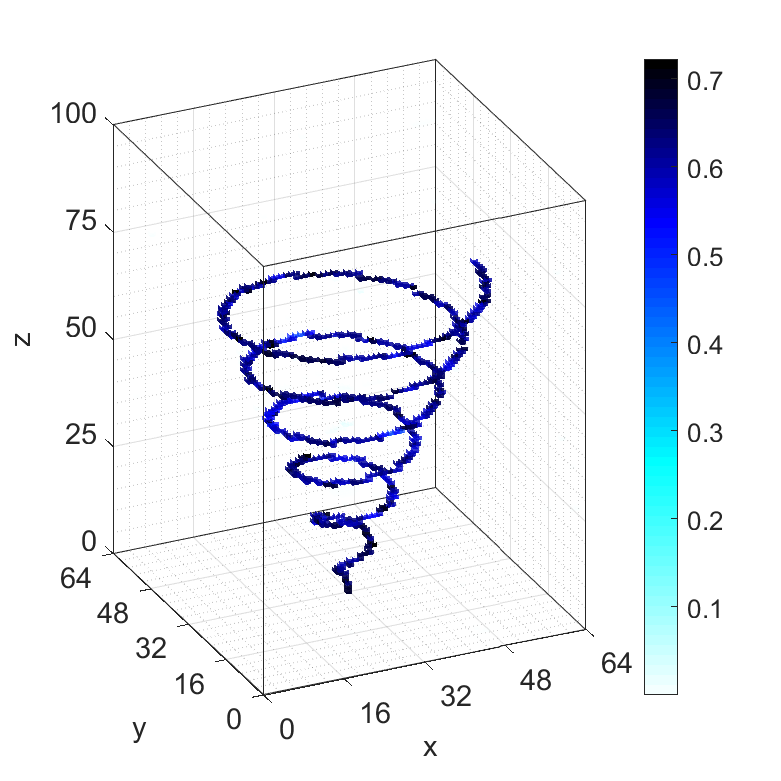
\includegraphics[width=0.33\columnwidth]{conhelix_complex_TwIST_3d}
    \caption{}
\end{subfigure}}
\caption{Experimental verification with phase-shifting holograms}
\label{fig_exp}
\end{figure}

\begin{table}[H]
\centering
\caption{\bf Specification of the Experiments}
\begin{tabular}{ccc}
\hline
Objects & $z$         & $\Delta x$ \\
\hline
Beads & $L_1(2L_1-1)$ & $\Phi_{i1}$ \\
Bio   & $L_2(2L_2-1)$ & $\Phi_{i2}$ \\
Point scatter  & $L_2(2L_2-1)$ & $\Phi_{i2}$ \\
\hline
\end{tabular}
\label{tb_expspec}
\end{table}

\subsection{Auto-focusing property of the proposed method}

\subsection{Analysis}

%====================================================================

\section{Conclusion}

In this work, we have presented .......

Interferometric based hologram can be processed to be a complex hologram.

%====================================================================

\section{Funding}

Brain Korea Plus 2019; 
% National Science Foundation of China~(NSFC)~(61705241).

% The authors thank H. Haase, C. Wiede, and J. Gabler for technical support.

%%%%%%%%%%%%%%%%%%%%%%%%%%%%%%%%%%%%%%%%%%%%%%%%%%%%%%%%%%%%%%%%%
\bibliography{3dholoref}

\bibliographyfullrefs{3dholoref}

\end{document}
